% Chapter 1

\chapter{Introducción general} % Main chapter title

\label{Chapter1} % For referencing the chapter elsewhere, use \ref{Chapter1} 
\label{IntroGeneral}

%----------------------------------------------------------------------------------------

% Define some commands to keep the formatting separated from the content 
\newcommand{\keyword}[1]{\textbf{#1}}
\newcommand{\tabhead}[1]{\textbf{#1}}
\newcommand{\code}[1]{\texttt{#1}}
\newcommand{\file}[1]{\texttt{\bfseries#1}}
\newcommand{\option}[1]{\texttt{\itshape#1}}
\newcommand{\grados}{$^{\circ}$}

%----------------------------------------------------------------------------------------
%\section{Introducción}
En este capítulo se realiza un acercamiento a los conceptos básicos del aprendizaje automático y financieros. Asimismo, se menciona el estado del arte en un buró de crédito argentino, y por último se explica la motivación, alcance y objetivos del presente trabajo.  
%----------------------------------------------------------------------------------------
\section{Inteligencia artificial en el ámbito financiero}

El sector financiero fué y sigue siendo uno de los pioneros a la hora de implementar inteligencia artificial, una de las tecnologías más revolucionarias de los últimos tiempos.

La inteligencia artificial se refiere a sistemas o máquinas que imitan la inteligencia humana para realizar tareas, mejorando iterativamente a partir de la recopilación de información. Su objetivo es mejorar significativamente las capacidades humanas.
 
Actualmente  la inteligencia artificial mejora el rendimiento y la productividad de las empresas mediante la automatización de los procesos y tareas que antes requerían esfuerzo humano o expertos dedicados a ello.
Hoy en día, muchas aplicaciones de inteligencia artificial son utilizadas tanto por instituciones tradicionales como por \textit{fintech} \cite{molina}. 


El \textit{score} o \textit{scoring} es un método estadístico que predice la probabilidad de \textit{default} o incumplimiento de pago. Se representa con un número que generalmente oscila entre 1 y 999 es el principal factor que analizan los prestamistas ante solicitudes de crédito. Un \textit{score} crediticio que utiliza inteligencia artificial es mucho más completo y sofisticado comparado con criterios tradicionales de \textit{score} de crédito.

En la figura \ref{fig:Figura3}\footnote{Imagen tomada de \url{https://www.bcra.gob.ar/Pdfs/Publicaciones/CreditScoring.pdf}} se observa que  la relación entre el \textit{score} (representado por "z") y el riesgo no es lineal, por lo que el cambio en el riesgo derivado de un cambio en el \textit{score} depende de los valores que este último tome. Para valores del \textit{score} muy bajos un aumento genera una rápida subida en la probabilidad de cumplimiento y una rápida disminución de la probabilidad de \textit{default}, mientras que para valores de \textit{score} altos, una mejora hace que la probabilidad de cumplimiento aumente poco y genera una leve caída en el riesgo.

\vspace{1cm}
\begin{figure}[htbp]
	\centering
	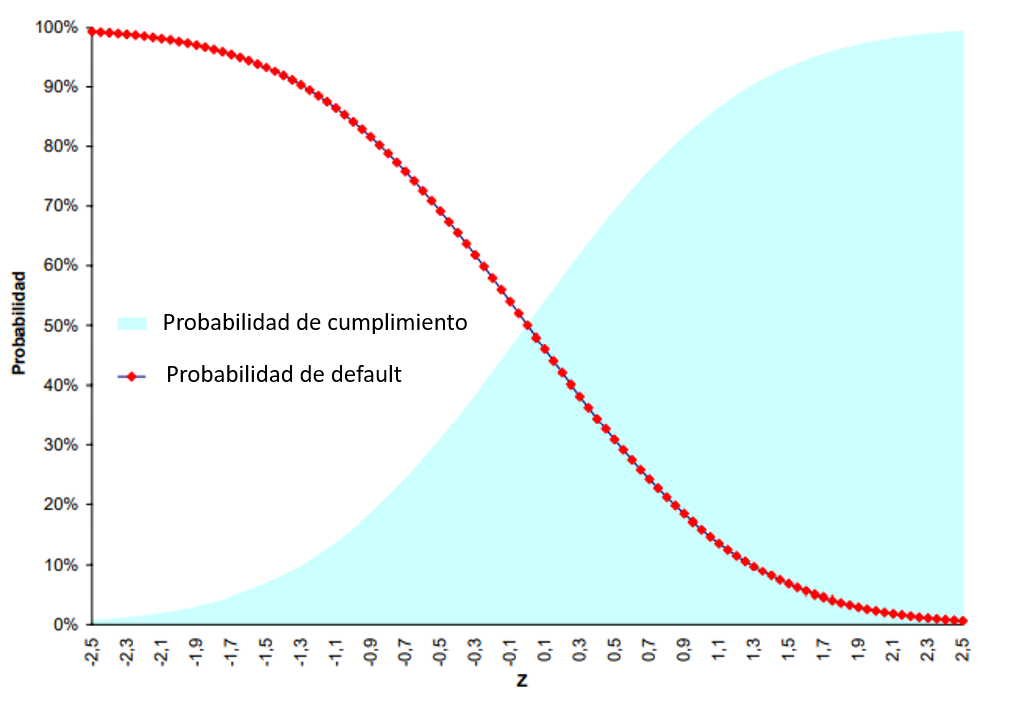
\includegraphics[width=0.8\textwidth]{./Figures/Figura3.png}
	\caption{Relación entre el \textit{score} y el riesgo. 						}
	\label{fig:Figura3}
\end{figure}
\vspace{1cm}

\vspace{1cm}


Los bancos digitales y \textit{fintech} utilizan algoritmos de aprendizaje de máquina cuya importancia radica en la objetividad y la eliminación de sesgos para la toma de decisiones. Asimismo, la capacidad de cómputo de este tipo de sistemas, permite manejar grandes cantidades de datos en poco tiempo y la computación cognitiva ayuda a administrar datos estructurados y no estructurados. Los algoritmos analizan historiales de transacciones e identifican a tiempo signos de futuros problemas.

%\subsection{Una introducción (no tan corta) a \LaTeX{}}

%\subsubsection{Una subsubsección}

%\subsection{Guía matemática rápida para \LaTeX{}}


%----------------------------------------------------------------------------------------

\section{Estado del arte: caso Nosis}

Nosis es una empresa fundada en la década del 80 con el objeto de brindar información de antecedentes comerciales, mercados financieros en línea y comercio exterior para aportar herramientas analíticas que faciliten la toma de decisiones.
Como buró, cuenta con bases de datos exclusivas, información compartida por más de 100 entidades, información pública tanto del BCRA, ANSES, AFIP, entre otros  e innovadoras técnicas analíticas con actualización constante de datos. 

Una de sus principales unidades de negocio trabaja sobre informes comerciales que tienen como variable principal un \textit{score} desarrollado por la misma empresa. 
El \textit{score} de Nosis es un ejemplo de un \textit{score} de riesgo. Brinda información sobre la probabilidad de \textit{default} o mora del cliente consultado desde el momento de la consulta propiamente dicha y 12 meses hacia adelante. Detrás de este número único o calificación, hay más de 70 variables de información dentro del algoritmo desarrollado por la empresa que puso en consideración el endeudamiento histórico de varias fuentes de información y más de 600 atributos de datos. El algoritmo se procesa en el momento de la consulta e indica que cuanto más alto sea el \textit{score}, existe una menor probabilidad de \textit{default} o mora.  
Las bases de datos con las que trabaja Nosis cubren el 99.99\% del endeudamiento de una persona o empresa con el sistema financiero total a nivel país. 

El presente trabajo se centró en el desarrollo de un \textit{score} interno con variables e información de los sistemas transaccionales de la compañía que, por un lado permita automatizar el proceso manual llevado a cabo por el área de finanzas y por el otro, permita evolucionar hacia una estrategia de política crediticia centrada en el comportamiento del cliente con la compañía. 

En la figura \ref{fig:Proceso actual}  se observa el proceso previo al desarrollo del presente trabajo.

\vspace{1cm}
\begin{figure}[htbp]
	\centering
	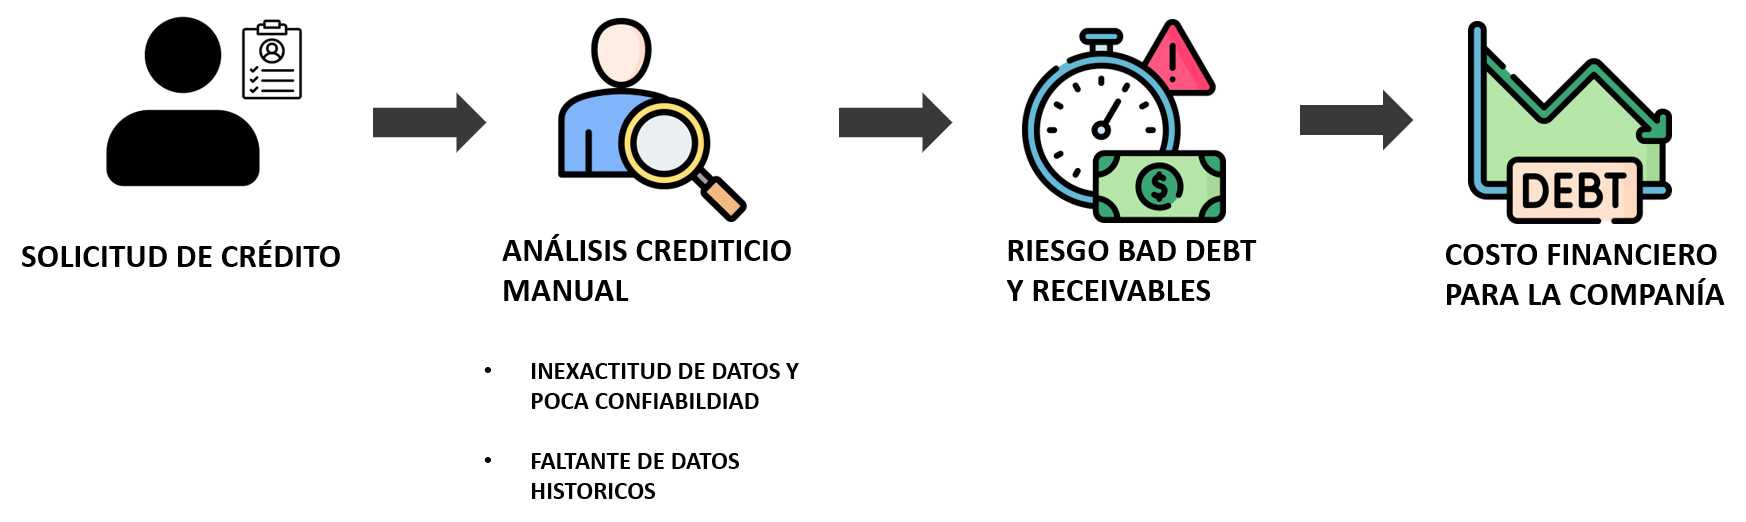
\includegraphics[width=1.0\textwidth]{./Figures/Figura2.png}
	\caption{Proceso previo a la automatización.}
	\label{fig:Proceso actual}
\end{figure}
\vspace{1cm}


%----------------------------------------------------------------------------------------

\section{Motivación}

%\subsection{Carpetas}

La principal motivación para la realización de este trabajo fue la eliminación de subjetividades en procesos de asignación de límite crediticio, la reducción de la deuda generada por los clientes morosos y la optimización del capital empleado (\textit{receivables}) para la generación de mejores resultados, otorgando un mejor servicio de crédito a los clientes, junto a la adopción de tecnologías relacionadas al análisis predictivo en una empresa tradicional de muchos años y con procesos establecidos adversos al cambio.

La no existencia de una herramienta que permita objetivamente asignar límite de crédito a cada cliente significaba un alto riesgo asociado a la mora o incobrabilidad. De hecho, durante el año 2021 el \textit{bad debt} o deuda incobrable ascendía casi al 30\% de la cartera de clientes con crédito. Por otro lado, la compañía no estaba cobrando interés alguno por los créditos cedidos y el P\&L de crédito (\textit{profit and loss}) arrojaba resultados negativos por un porcentaje considerable de clientes en mora sin un ROIC (\textit{return on invested capital})asociado.

En referencia a la opinión de los clientes en temáticas de crédito, se obtuvo un bajo NPS (\textit{net promoter score}) en las encuestas de satisfacción de servicio enviadas.
Sumado a lo anteriormente mencionado, se encontraban a menudo errores manuales en análisis o asignaciones de crédito  por causa de la no automatización de procesos. Existía la dependencia de personal específico solo para realizar un análisis de riesgo de cada cliente a partir de reglas de negocio definidas.

El presente trabajo fue el primer algoritmo desarrollado por el área de \textit{data analytics} y el principal caso de uso dentro de la compañía, rompiendo así la brecha entre las áreas de negocio y de TI (tecnología de la información).


%----------------------------------------------------------------------------------------

\section{Objetivos y alcance}

\subsection{Objetivos}

El propósito de este trabajo consistió esencialmente en el diseño, pruebas e implementación de una solución de inteligencia artificial que permite estimar la mora
y la rotación del crédito de los clientes activos de la compañía, asegurando a una mejor distribución de los recursos crediticios, considerando distintos aspectos del cliente en cuanto a compras, pagos atrasados, deuda total vigente, cheques rechazados, antigüedad e historial de pagos, entre otras variables.

En la figura \ref{fig:Diagrama en bloques del sistema}  se observa un diagrama general de la solución y las etapas que la componen.

\vspace{1cm}
\begin{figure}[htbp]
	\centering
	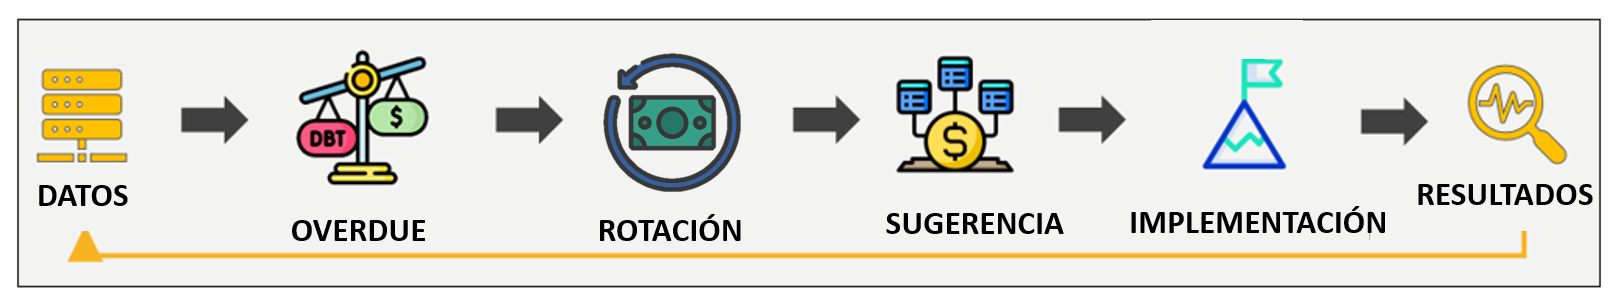
\includegraphics[width=1.0\textwidth]{./Figures/Diagrama de FlujoV2.png}
	\caption{Diagrama en bloques del sistema.}
	\label{fig:Diagrama en bloques del sistema}
\end{figure}
\vspace{1cm}

En el capítulo \ref{Chapter3} se detalla el diseño y la implementación de las etapas que componen este sistema.

	
\subsection{Alcance}


El alcance de este trabajo estuvo orientado a desarrollar una solución de software que permite cubrir aspectos que giran en torno a los siguientes ejes:

\begin {enumerate}
\item Entendimiento del problema: 
	\begin {itemize}
	\item \textit{assesment} del proceso de asignación manual del límite de
crédito. 
	\item definición de expectativas post implementación de la solución.
	\end {itemize}

	
\item Aspectos relacionados al entendimiento del negocio: 
	\begin {itemize}
	\item entendimiento de las restricciones asociadas al proceso. 
	\item entendimiento de aspectos generales del negocio.
	\end {itemize}
	
\item Aspectos relacionados a la adquisición y comprensión de datos: 
	\begin {itemize}
	\item \textit{assesment} de las fuentes de datos (modelos en \textit{datawarehouse} y otras). 
	\item exploración de los datos para determinar la calidad de la información.
	\end {itemize}
	
\item Aspectos relacionados al modelado: 
	\begin {itemize}
	\item diseño de características: generación de variables adicionales a partir de los datos sin procesar para facilitar 
el entrenamiento del modelo.
	\item entrenamiento del modelo: elección del modelo que responda a la pregunta de negocio con la máxima precisión, evaluando métricas de éxito.
	\end {itemize}
	
\item Aspectos relacionados al despliegue: 
	\begin {itemize}
	\item implementación del/los modelo/s en un entorno de producción o similar para el consumo por el usuario final o aplicaciones. 
	\end {itemize}
\end {enumerate}
 
El alcance de este trabajo no cubre:
\begin {itemize}
\item el mantenimiento de la base de datos en la cual se aloja la información generadora de la entrada para el modelo de inteligencia artificial.
\item la instalación y mantenimiento del \textit{hardware} necesario para el procesamiento de información del modelo desarrollado.
\item la disponibilización de la salida del algoritmo directamente en alguna aplicación de la compañía.
\end {itemize}